\section{Results}
\label{sec:results}
This section presents an evaluation of our results and a discussion of the model's performance. We begin with a visual comparison between an estimated and ground-truth pose, followed by a detailed analysis of the model's performance on the test set. Finally, we examine the resulting trajectories from our localization pipeline. 

\subsection{Visual Comparison of Estimated and Ground Truth Pose}
Figure \ref{fig:pose-comparison} illustrates a visual comparison between the estimated pose and the corresponding ground-truth from the test set, shown from four perspectives rotated at 0°, 90°, 180° and 270° angles. Overall, the estimated pose captures the global body posture of the target well. In particular, the global orientation of the skeleton and the left-leg joint positions align closely with the ground-truth. However, discrepancies are visible in the right lower leg, which appears shifted further back relative to the ground-truth. Furthermore, the estimated upper body exhibits a slightly stronger forward lean than the reference.

\begin{figure}[htbp]
    \centering
    \includegraphics[width=0.8\columnwidth]{img/pose_comparison.pdf}
    \caption{Comparison of a single estimated 3D pose (red) to its corresponding ground-truth pose (blue) from four different perspectives.}
    \Description{}
    \label{fig:pose-comparison}
\end{figure}

\subsection{Metrics}
Our recorded metrics for the test set mirror the results of the visual comparison. Figure \ref{fig:mjpe} shows the Mean Joint Position Error (MJPE) for all items from the test set. The hip was the easiest joint to estimate with about 2~cm median error. The local coordinate system from MediaPipe starts from the hip which reduces the possible space to two dimensions, making the estimation a lot easier. On the other hand the most outer joints, the wrist and ankle, which are further away and move the most in space, performed the worst, with a median of approximately 5~cm and 7~cm and a bigger IQR. For all joints 75\% of the estimations are within 12~cm. Given how complex a pose can be, especially with rotation included, this is not just predicting a mean pose. 
\todo{we should mention our trainmetrics right?} %To see how model training performed and overfitting and stuff for transparency? 

Secondly, while most of the data has a reasonable error, there is a significant portion with higher errors. We explained this for two reasons: There are poses which have a signal, but no history information available when the subject has just entered the SensFloor which gives the model not enough information to estimate an accurate pose and when the subject performs an unforseen action, for example by rapidly changing the directions or moving their body unnaturally, e.g. looking at their watch, fixing sweater. 

Thirdly, there is a tiny mismatch between the left and right side of the joints. We concluded this mismatch to stem from the targets themselves. As MediaPipe does not provide 100\% accurate targets, the specific setup of our data collection could influence the outcome.  

\begin{figure}[htbp]
    \centering
    \includegraphics[width=\columnwidth]{img/mjpe_boxplot.pdf}
    \caption{Boxplot of Mean Joint Position Error for each joint on test set with $n=21898$ samples. The box is the Interquartile Range (IQR) and the Whiskers mark the $5^{th}$ and $95^{th}$ percentile.}
    \Description{}
    \label{fig:mjpe}
\end{figure}

Furthermore the figure explains the big difference for the results of the Percentage Correct Key points (PCK) between a 5~cm and 10~cm threshold on the ankles.
As the Interquartile range for the MJPE of the feet ankles lay just above 5~cm the PCK for this threshold is $37\%$ where for 10~cm it is $72\%$.
The mean PCK for 5~cm is $61\%$ and for 10~cm it is $87\%$.
\todo{should we Maybe the val\_loss graph or sth would be nice}
The other values and the training graph can be found in the annex.

% - Predicted pose compared to true pose image
% - Training metrics (boxplot and mention pck) explain tha numbers


% - Estimated position (House of Kalmann)
\subsection{Localization and Kalman-Filter Effect}
In \ref{subsec:localization}, we introduced our approach for extracting information about the person's current global position from the SensFloor activation signals. The left side of Figure \ref{fig:kalman-filter-effect} shows the raw clustering position trajectory we recorded during a test walk. The illustrated trajectory is highly erratic. This instability is caused by two main factors. First, the algorithm creates jumps in the estimated position as the mean shifts abruptly whenever a foot makes or breaks contact with the floor. Second, the SensFloor fields produce significant background noise, even in areas where no activity takes place. While increasing the noise signal threshold suppresses some of the noise, it is not a universal solution, as signal intensity of people moving on the floor varies depending on the person's footwear. 

However, applying the Kalman filter largely reduces these issues, as illustrated on the right side of Figure \ref{fig:kalman-filter-effect}. By smoothing out the abrupt transitions and mitigating the impact of outliers, the filter produces a smooth and, according to our empirical evaluation, accurate trajectory.

\todo{set the arrows to a fixed size, so it's not confusing}
\begin{figure}[htbp]
    \centering
    \includegraphics[width=\columnwidth]{img/kalman-filter-effect.pdf}
    \caption{Comparison of raw (left) and filtered (right) localization trajectories. The arrows indicate the direction of the movement.}
    \Description{}
    \label{fig:kalman-filter-effect}
\end{figure}
% - Inference works



% - evaluation
    % - Mediapipe inconsistency
    % - Only male subjects for training
    % - No groundtruth for kalman filter
    % - test set split? No evaluation that our test and trianing set have a similar distribution
    % - Model learned to Look down
    % - Only small sequences of walking possible due to the small floor (and missing API endpoint with good estimations probably)
    % - Very limited training set with 